% Options for packages loaded elsewhere
\PassOptionsToPackage{unicode}{hyperref}
\PassOptionsToPackage{hyphens}{url}
%
\documentclass[
  ignorenonframetext,
  aspectratio=43,
]{beamer}
\usepackage{pgfpages}
\setbeamertemplate{caption}[numbered]
\setbeamertemplate{caption label separator}{: }
\setbeamercolor{caption name}{fg=normal text.fg}
\beamertemplatenavigationsymbolshorizontal
% Prevent slide breaks in the middle of a paragraph
\widowpenalties 1 10000
\raggedbottom
\setbeamertemplate{part page}{
  \centering
  \begin{beamercolorbox}[sep=16pt,center]{part title}
    \usebeamerfont{part title}\insertpart\par
  \end{beamercolorbox}
}
\setbeamertemplate{section page}{
  \centering
  \begin{beamercolorbox}[sep=12pt,center]{part title}
    \usebeamerfont{section title}\insertsection\par
  \end{beamercolorbox}
}
\setbeamertemplate{subsection page}{
  \centering
  \begin{beamercolorbox}[sep=8pt,center]{part title}
    \usebeamerfont{subsection title}\insertsubsection\par
  \end{beamercolorbox}
}
\AtBeginPart{
  \frame{\partpage}
}
\AtBeginSection{
  \ifbibliography
  \else
    \frame{\sectionpage}
  \fi
}
\AtBeginSubsection{
  \frame{\subsectionpage}
}

\usepackage{amsmath,amssymb}
\usepackage{lmodern}
\usepackage{iftex}
\ifPDFTeX
  \usepackage[T1]{fontenc}
  \usepackage[utf8]{inputenc}
  \usepackage{textcomp} % provide euro and other symbols
\else % if luatex or xetex
  \usepackage{unicode-math}
  \defaultfontfeatures{Scale=MatchLowercase}
  \defaultfontfeatures[\rmfamily]{Ligatures=TeX,Scale=1}
\fi
\usetheme[]{default}
\usecolortheme{default}
% Use upquote if available, for straight quotes in verbatim environments
\IfFileExists{upquote.sty}{\usepackage{upquote}}{}
\IfFileExists{microtype.sty}{% use microtype if available
  \usepackage[]{microtype}
  \UseMicrotypeSet[protrusion]{basicmath} % disable protrusion for tt fonts
}{}
\makeatletter
\@ifundefined{KOMAClassName}{% if non-KOMA class
  \IfFileExists{parskip.sty}{%
    \usepackage{parskip}
  }{% else
    \setlength{\parindent}{0pt}
    \setlength{\parskip}{6pt plus 2pt minus 1pt}}
}{% if KOMA class
  \KOMAoptions{parskip=half}}
\makeatother
\usepackage{xcolor}
\newif\ifbibliography
\setlength{\emergencystretch}{3em} % prevent overfull lines
\setcounter{secnumdepth}{-\maxdimen} % remove section numbering


\providecommand{\tightlist}{%
  \setlength{\itemsep}{0pt}\setlength{\parskip}{0pt}}\usepackage{longtable,booktabs,array}
\usepackage{calc} % for calculating minipage widths
\usepackage{caption}
% Make caption package work with longtable
\makeatletter
\def\fnum@table{\tablename~\thetable}
\makeatother
\usepackage{graphicx}
\makeatletter
\def\maxwidth{\ifdim\Gin@nat@width>\linewidth\linewidth\else\Gin@nat@width\fi}
\def\maxheight{\ifdim\Gin@nat@height>\textheight\textheight\else\Gin@nat@height\fi}
\makeatother
% Scale images if necessary, so that they will not overflow the page
% margins by default, and it is still possible to overwrite the defaults
% using explicit options in \includegraphics[width, height, ...]{}
\setkeys{Gin}{width=\maxwidth,height=\maxheight,keepaspectratio}
% Set default figure placement to htbp
\makeatletter
\def\fps@figure{htbp}
\makeatother

\usepackage{ragged2e}
\usepackage{etoolbox}

\apptocmd{\frame}{}{\justifying}{} 

\setbeamertemplate{enumerate items}[default]
\setbeamertemplate{itemize items}[circle]
\setbeamersize{text margin left=2.25em, text margin right=2.25em}

\let\OLDitemize\itemize
\renewcommand\itemize{
    \OLDitemize\addtolength{\itemsep}{3pt plus 1pt minus 1pt}
}
\let\OLDenumerate\enumerate
\renewcommand\enumerate{
    \OLDenumerate\addtolength{\itemsep}{3pt plus 1pt minus 1pt}
}

\usepackage{orcidlink}
\usepackage{amsmath}
\DeclareMathOperator*{\argmax}{argmax}

\makeatletter
\def\@listii{\leftmargin\leftmarginii
              \topsep    1ex
              \parsep    0\p@   \@plus\p@
              \itemsep   \parsep}
\makeatother

\usepackage{lipsum}

\let\olditem\item
\renewcommand\item{\olditem\justifying}

\definecolor{blue}{RGB}{0,114,178}
\definecolor{red}{RGB}{213,94,0}
\definecolor{yellow}{RGB}{240,228,66}
\definecolor{green}{RGB}{0,158,115}

\definecolor{MyBackground}{RGB}{255,253,218}

\setbeamercolor{section in toc}{fg=blue}
\setbeamercolor{subsection in toc}{fg=red}

\setbeamercolor{frametitle}{fg=blue}
\setbeamercolor{title}{fg=blue}

\setbeamertemplate{footline}[frame number]
\setbeamertemplate{navigation symbols}{} 
\setbeamertemplate{itemize items}{-}

\setbeamercolor{itemize item}{fg=blue}
\setbeamercolor{itemize subitem}{fg=blue}
\setbeamercolor{enumerate item}{fg=blue}
\setbeamercolor{enumerate subitem}{fg=blue}
\setbeamercolor{button}{bg=MyBackground,fg=blue}

\newcounter{daggerfootnote}
\newcommand*{\daggerfootnote}[1]{%
    \setcounter{daggerfootnote}{\value{footnote}}%
    \renewcommand*{\thefootnote}{\fnsymbol{footnote}}%
    \footnote[2]{#1}%
    \setcounter{footnote}{\value{daggerfootnote}}%
    \renewcommand*{\thefootnote}{\arabic{footnote}}%
}

\AtBeginSection{
    \begingroup
    \setbeamercolor{background canvas}{bg=yellow}
    \begin{frame}
        \begin{centering}
            \usebeamerfont{section title}\huge\color{black}\insertsection\par
        \end{centering}
    \end{frame}
    \endgroup
}
\makeatletter
\makeatother
\makeatletter
\makeatother
\makeatletter
\@ifpackageloaded{caption}{}{\usepackage{caption}}
\AtBeginDocument{%
\ifdefined\contentsname
  \renewcommand*\contentsname{Table of contents}
\else
  \newcommand\contentsname{Table of contents}
\fi
\ifdefined\listfigurename
  \renewcommand*\listfigurename{List of Figures}
\else
  \newcommand\listfigurename{List of Figures}
\fi
\ifdefined\listtablename
  \renewcommand*\listtablename{List of Tables}
\else
  \newcommand\listtablename{List of Tables}
\fi
\ifdefined\figurename
  \renewcommand*\figurename{Figure}
\else
  \newcommand\figurename{Figure}
\fi
\ifdefined\tablename
  \renewcommand*\tablename{Table}
\else
  \newcommand\tablename{Table}
\fi
}
\@ifpackageloaded{float}{}{\usepackage{float}}
\floatstyle{ruled}
\@ifundefined{c@chapter}{\newfloat{codelisting}{h}{lop}}{\newfloat{codelisting}{h}{lop}[chapter]}
\floatname{codelisting}{Listing}
\newcommand*\listoflistings{\listof{codelisting}{List of Listings}}
\makeatother
\makeatletter
\@ifpackageloaded{caption}{}{\usepackage{caption}}
\@ifpackageloaded{subcaption}{}{\usepackage{subcaption}}
\makeatother
\makeatletter
\@ifpackageloaded{tcolorbox}{}{\usepackage[many]{tcolorbox}}
\makeatother
\makeatletter
\@ifundefined{shadecolor}{\definecolor{shadecolor}{rgb}{.97, .97, .97}}
\makeatother
\makeatletter
\makeatother
\ifLuaTeX
  \usepackage{selnolig}  % disable illegal ligatures
\fi
\IfFileExists{bookmark.sty}{\usepackage{bookmark}}{\usepackage{hyperref}}
\IfFileExists{xurl.sty}{\usepackage{xurl}}{} % add URL line breaks if available
\urlstyle{same} % disable monospaced font for URLs
\hypersetup{
  pdftitle={Seminar 3},
  pdfauthor={Gabriel E. Cabrera Guzmán},
  hidelinks,
  pdfcreator={LaTeX via pandoc}}

\title[Seminar 3]{Seminar
3\daggerfootnote{\texttt{gabriel.cabreraguzman@postgrad.manchester.ac.uk}}}
\subtitle{Probability Theory 1 \& 2 (Concepts \& Rules)}
\author[Gabriel E. Cabrera Guzmán]{
    {Gabriel E. Cabrera
Guzmán\textsuperscript{\normalsize\orcidlink{0000-0000-0000-0000}}} \medskip
}
\date{October 18, 2025}
\institute[]{
    The University of Manchester\\
Alliance Manchester Business School \bigskip
}

\definecolor{quarto-callout-note-color}{RGB}{0,114,178}
\definecolor{quarto-callout-note-color-frame}{RGB}{0,114,178}
\definecolor{quarto-callout-warning-color}{RGB}{213,94,0}
\definecolor{quarto-callout-warning-color-frame}{RGB}{213,94,0}
\begin{document}
\frame{\titlepage}
\ifdefined\Shaded\renewenvironment{Shaded}{\begin{tcolorbox}[interior hidden, borderline west={3pt}{0pt}{shadecolor}, breakable, sharp corners, enhanced, boxrule=0pt, frame hidden]}{\end{tcolorbox}}\fi

\begin{frame}{Exercise 1}
\protect\hypertarget{exercise-1}{}
\begin{enumerate}
\item
  A university has three residences for students. The first has 500
  single study bedrooms, the second has 1000 and the third has 2000.
  When a student is allocated randomly to a residence, what is the
  probability of the second residence?

  \pause

  \[
   \begin{aligned}
   \text{Pr}(\textit{Second Residence}) & = \frac{n(\textit{Second Residence})}{n(\textit{Total})} \\
                                        & = \frac{1000}{500 + 1000 + 2000} 
                                          = \frac{1000}{3500} 
                                          = \frac{2}{7}
   \end{aligned}
   \]
\end{enumerate}
\end{frame}

\begin{frame}{Exercise 1 (Cont'd)}
\protect\hypertarget{exercise-1-contd}{}
\begin{enumerate}
\setcounter{enumi}{1}
\item
  Five men and three women are short-listed for a job. What is the
  probability that a man gets the job? What assumption do you need to
  make to calculate the probability?

  \[
   \text{Pr}(\textit{Man}) = \frac{n(\textit{Man})}{n(\textit{Total Short - listed})} = \frac{5}{5 + 3} = \frac{5}{8}  
   \]

  \vspace{5pt}

  We assume that the chance of each person to get the job is the
  \textbf{same}. That is, the events of the job taken by each of these
  eight candidates are \textbf{equally} likely.
\end{enumerate}
\end{frame}

\begin{frame}{Exercise 2}
\protect\hypertarget{exercise-2}{}
In a particular city 20\% of people subscribe to the morning newspaper,
30\% to the evening newspaper and 10\% subscribe to both. Determine the
probability that an individual from this city subscribes to the morning
newspaper or the evening newspaper or both. Are the events, `subscribe
to morning newspaper', and `do not subscribe to morning newspaper'
mutually exclusive or not? Say why or why not.

\pause

\textbf{A:} Define set \(A\) as people who subscribe to the morning
newspaper and set \(B\) as people who subscribe to the evening
newspaper.

We are told \(\Pr(A) = 0.20\), \(\Pr(B) = 0.30\), and
\(\Pr(A \cap B) = 0.10\).\\
To find \(\Pr(A \cup B)\), we can use the inclusion--exclusion rule as
follows:

\[
\begin{aligned}
\Pr(A \cup B) & = \Pr(A) + \Pr(B) - \Pr(A \cap B) \\
              & = 0.20 + 0.30 - 0.10 \\
              & = 0.40 
\end{aligned}
\]
\end{frame}

\begin{frame}{Exercise 2 (Cont'd)}
\protect\hypertarget{exercise-2-contd}{}
In the above notation, \(A \cap B\) means both events \(A\) \textbf{and}
\(B\) have occurred (the person subscribes to both morning and evening
newspapers), and \(A \cup B\) means either \(A\) \textbf{or} \(B\) or
\textbf{both} has occurred (the person subscribes either to both morning
or to evening newspapers \textbf{or both}).

The events \(A\) (subscribe to the morning newspaper) and \(Not \; A\)
(not subscribe to the morning newspaper) are \textbf{mutually exclusive}
because they cannot happen simultaneously. In other words:

\[
\Pr(A \cap Not \; A) = 0
\]
\end{frame}

\begin{frame}{Exercise 3}
\protect\hypertarget{exercise-3}{}
A taxi company runs 4 taxis. Two are older and the probability that a
particular one of these breaks down on a particular day is 0.1. The
other two are newer and the probability that a particular one breaks
down on a particular day is 0.05. On a particular day: \vspace{10pt}

\pause

\begin{itemize}
\item
  Define A as the event that the first old taxi breaks down
\item
  Define B as the event that the second old taxi breaks down
\item
  Define C as the event that the first new taxi breaks down
\item
  Define D as the event that the second new taxi breaks down
\end{itemize}
\end{frame}

\begin{frame}{Exercise 3 (Cont'd)}
\protect\hypertarget{exercise-3-contd}{}
\begin{enumerate}
\item
  What is the probability that all 4 taxis break down? State any
  assumptions you make.

  \pause

  \textbf{A:} Assuming that events A, B, C, D are all
  \textbf{independent}, the probability that all 4 taxis break down is:

  \[
   \begin{aligned}
   \Pr(\textit{All Break Down}) &= \Pr(A \; and \; B \; and \; C \; and \; D) \\
   & = \Pr(A)\Pr(B)\Pr(C)\Pr(D) \\
   & = 0.1 \times 0.1 \times 0.05 \times 0.05 \\
   & = 0.000025
   \end{aligned}
   \]
\end{enumerate}
\end{frame}

\begin{frame}{}
\protect\hypertarget{section}{}
\begin{enumerate}
\setcounter{enumi}{1}
\item
  What is the probability that the two newer taxis break down but the
  older ones continue to work?

  \pause

  \textbf{A:} The probability that the two newer taxis break down but
  the older ones continue to work is

  \[
   \begin{aligned}
   & \Pr(\textit{Old not Break Down and New Break Down}) \\ 
   & = \Pr(Not \; A \; and \; Not \; B \; and \; C \; and \; D) \\
   & = \Pr(Not \; A)\Pr(Not \; B)\Pr(C)\Pr(D) \\
   & = (1 - 0.1) \times (1 - 0.1) \times 0.05 \times 0.05 \\
   & = 0.9 \times 0.9 \times 0.05 \times 0.05 \\
   & = 0.002025
   \end{aligned}
   \]
\end{enumerate}
\end{frame}

\begin{frame}{Exercise 4}
\protect\hypertarget{exercise-4}{}
Consider the data in the contingency table below, giving the number of
male and female students on various degree courses in the business
school of a university. There are 1500 students in total. \vspace{-5pt}

\[
\footnotesize
\begin{array}{lcccc}
\toprule
 & \textbf{Accountancy} & \textbf{Economics} & \textbf{Finance} & \textbf{Business Information} \\
\midrule
\text{Male}   & 330 & 360 & 90 & 120 \\
\text{Female} & 120 & 390 & 60 & 30 \\
\bottomrule
\end{array}
\]

\vspace{10pt}

Calculate the following probabilities:

\begin{enumerate}
\tightlist
\item
  The probability that a student takes Economics.
\end{enumerate}

\pause

\[
\Pr(\text{Economics}) = \frac{750}{1500} = \frac{1}{2} = 0.50
\]
\end{frame}

\begin{frame}{Exercise 4 (Cont'd)}
\protect\hypertarget{exercise-4-contd}{}
\begin{enumerate}
\setcounter{enumi}{1}
\item
  The probability that \textbf{a female} student takes Economics.

  \pause

  \[
  \begin{aligned}
  \Pr(\textit{Economics} \, | \, \textit{Female}) & = \frac{\Pr(\textit{Economics}\cap\textit{Female})}{\Pr(Female)} \\ & = \frac{\frac{390}{1500}}{\frac{600}{1500}} = 0.65 \\
  \end{aligned}
  \]
\item
  The probability that a student is female \textbf{and} takes Economics.

  \pause

  \[
  \begin{aligned}
  \Pr(\textit{Economics} \, \cap \, \textit{Female}) & = \frac{n(\textit{Economics} \cap \textit{Female})}{n(\textit{Total})} \\ & = \frac{390}{1500} = 0.26 \\
  \end{aligned}
  \]
\end{enumerate}
\end{frame}

\begin{frame}{}
\protect\hypertarget{section-1}{}
\begin{enumerate}
\setcounter{enumi}{3}
\item
  The probability that a student takes Economics \textbf{given that}
  they are female:

  \pause

  This is the same as part b
\item
  The probability that \textbf{a Finance} student is female.

  \pause

  \[
  \begin{aligned}
  \Pr(\textit{Female}\,| \,\textit{Finance}) & = \frac{\Pr(\textit{Female} \cap \textit{Finance})}{\Pr(\textit{Finance})} \\ & = \frac{\frac{60}{1500}}{\frac{150}{1500}} = \frac{60}{150}= 0.4
  \end{aligned}
  \]
\end{enumerate}
\end{frame}

\begin{frame}{}
\protect\hypertarget{section-2}{}
\begin{enumerate}
\setcounter{enumi}{5}
\item
  The probability that a student is female given that they do Finance.

  \pause

  This is the same as part e.
\item
  Are the events 'student is female' and `student takes Economics'
  independent or not? Explain your answer.

  \pause

  We know that
  \(\Pr(\textit{Economics}\, | \, \textit{Female}) = 0.65\),
  \(\Pr(\textit{Economics}) = 0.50\). Since
  \(\Pr(\textit{Economics}\, | \, \textit{Female}) \neq \Pr(\textit{Economics})\),
  we conclude that two events are not independent (i.e.~they are
  dependent).
\end{enumerate}
\end{frame}

\begin{frame}{Exercise 5}
\protect\hypertarget{exercise-5}{}
A software company surveyed office managers to determine the probability
that they would buy a new graphics package; 80\% of the managers said
they would buy the package. Of these, 40\% were also interested in
upgrading their computer hardware. Among those managers who were not
interested in purchasing the graphics package only 10\% were interested
in upgrading their computer hardware.

Denote event B, ``manager would buy package'' and event U, ``manager
would upgrade''.
\end{frame}

\begin{frame}{Exercise 5 (Cont'd)}
\protect\hypertarget{exercise-5-contd}{}
\begin{enumerate}
\item
  Write down the percentage information supplied above in terms of
  probabilities and the events B, Not B, U and Not U.

  \pause

  \begin{itemize}
  \item
    Define event B as the manager would Buy the package
  \item
    Define event U as manager would Upgrade the hardware.
  \end{itemize}

  Unconditional probabilities: the question text said that 80\% of the
  managers would buy the package. Hence, \(\Pr(B) = 80\%\) and
  \(\Pr(Not \, B) = 20\%\).

  Conditional probabilities: the question text said that among these
  (managers who buy), 40\% were also interested in upgrading their
  computer hardware. Hence, \(\Pr(U|B) = 40\%\) and
  \(\Pr(Not \, U \,| \,B)=60\%\). In addition, the question text said
  that of those managers who were not interested in buying only 10\%
  were interested in upgrading. Hence, \(\Pr(U \, | \, Not\, B)=10\%\)
  and \(\Pr(Not\, U \, |Not\, B)=90\%\).
\end{enumerate}
\end{frame}

\begin{frame}{}
\protect\hypertarget{section-3}{}
\begin{enumerate}
\setcounter{enumi}{1}
\item
  Using a tree diagram or otherwise calculate the probability that an
  office manager who is interested in upgrading is also interested in
  purchasing the new graphics package.

  \textbf{A:} The probability that an office manager \textbf{who is
  interested in upgrading (conditional term)} is also interested in
  buying the new graphics package is \(\Pr(B\,|\,U)\). By using the
  definition and values derived in the tree diagram, we can find this
  condition probability as follows:

  \[
   \Pr(B\,|\,U) = \frac{\Pr(B \cap U)}{\Pr(U)} = \frac{32\%}{32\% + 2\%} = \frac{32}{34} = 0.94
   \]
\end{enumerate}
\end{frame}

\begin{frame}{}
\protect\hypertarget{section-4}{}
\vspace{10pt}

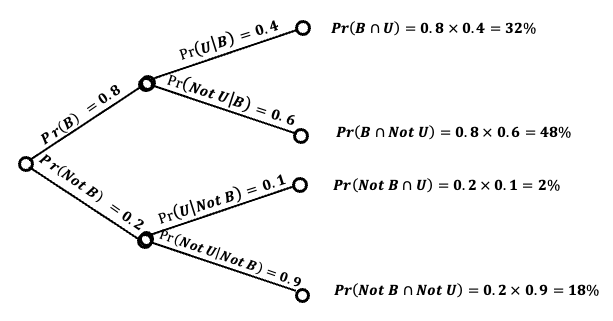
\includegraphics{Fig/q5_tree.png}
\end{frame}

\begin{frame}{Exercise 6}
\protect\hypertarget{exercise-6}{}
Students are given 3 chances to pass a professional examination. A
student who has passed is selected at random. The probability
distribution of X, the attempt number at which this student passed is
given as \vspace{-5pt}

\[
P(x) = \frac{0.4^{x -1} 0.6}{0.936} \quad \text{for} \; x = 1,2 \; \text{and} \; 3
\]

Write out the probability distribution of X. What proportion of students
pass at the third (i.e.~final) attempt?
\end{frame}

\begin{frame}{Exercise 6 (Cont'd)}
\protect\hypertarget{exercise-6-contd}{}
\textbf{A:} The probability distribution formula is given as follows:

\[
P(x) = \frac{0.4^{x -1} 0.6}{0.936}
\]

\vspace{5pt}

which presents the probability of passing the exam at attempt \(x\).
Substitute \(x = 1, 2, 3\) and find:

\[
\begin{aligned}
P(1) &= \frac{0.4^{1 -1} 0.6}{0.936} = \frac{1 \times 0.6}{0.936} = 0.6410 \\
P(2) &= \frac{0.4^{2 -1} 0.6}{0.936} = \frac{0.4 \times 0.6}{0.936} = 0.2564 \\
P(3) &= \frac{0.4^{3 -1} 0.6}{0.936} = \frac{0.4^2 \times 0.6}{0.936} = 0.1026
\end{aligned}
\]
\end{frame}

\begin{frame}{}
\protect\hypertarget{section-5}{}
Hence, we have the following probability distribution:

\[
\begin{array}{c|c}
\toprule
\textbf{x} & \textbf{Pr}(x) \\
\midrule
1 & 0.6410 \\
2 & 0.2564 \\
3 & 0.1026 \\
\bottomrule
\end{array}
\]

Therefore, 10.26\% of students pass the exam at the third attempt.
\end{frame}

\begin{frame}{Exercise 7}
\protect\hypertarget{exercise-7}{}
Two courier firms are competing for a contract to deliver in the City of
London for an investment company. Both have provided figures, based on
historic data, for the probability of delivery times of \(\frac{1}{2}\),
1, \(1 \frac{1}{2}\) and 2 hours.

Calculate the mean and variance of the delivery time for both courier
firms. Based on these which would you employ and why?
\end{frame}

\begin{frame}{Exercise 7 (Cont'd)}
\protect\hypertarget{exercise-7-contd}{}
\textbf{A:} We want to calculate the mean and variance of a random
variable (delivery time for two courier firms) using the following
table. We expand the table by adding two columns \(xP(x)\) and
\(x^2 P(x)\):

\vspace{-10pt}

\[
\centering
\tiny
\begin{array}{c|ccc|c|ccc}
\toprule
\multicolumn{4}{c|}{\textbf{Firm A}} & \multicolumn{4}{c}{\textbf{Firm B}} \\
\midrule
x & \Pr(x) & x\Pr(x) & x^{2}\Pr(x) & x & \Pr(x) & x\Pr(x) & x^{2}\Pr(x) \\
\midrule
0.5 & 0.6 & 0.3 & 0.5^{2}\times0.6=0.15 & 0.5 & 0.1 & 0.05 & 0.5^{2}\times0.1=0.025 \\
1   & 0.1 & 0.1 & 1^{2}\times0.1=0.10   & 1   & 0.7 & 0.7  & 1^{2}\times0.7=0.70 \\
1.5 & 0.1 & 0.15 & 1.5^{2}\times0.1=0.225 & 1.5 & 0.15 & 0.225 & 1.5^{2}\times0.15=0.3375 \\
2   & 0.2 & 0.4 & 2^{2}\times0.2=0.80   & 2   & 0.05 & 0.10 & 2^{2}\times0.05=0.20 \\
\midrule
\textbf{Sum} & 1 & 0.95 & 1.275 & & 1 & 1.075 & 1.2625 \\
\bottomrule
\end{array}
\]
\end{frame}

\begin{frame}{}
\protect\hypertarget{section-6}{}
\begin{itemize}
\item
  Firm A:

  We calculate the \(E(X)\) and \(E(X^2)\) as follows:

  \[
    \begin{aligned}
    \mu = E(X) &= \sum X \times P(x) = 0.95 \\ 
    E(X^2) &= \sum X^2 \times P(x) = 1.275
    \end{aligned}
    \]

  Therefore, using the formula for mean and variance we find that
  \vspace{-12.5pt}

  \[
    \begin{aligned}
    \mu &= 0.95 \\ 
    Var(X) &= E(X^2) - \mu^2 = 1.275 - 0.95^2 = 0.3725
    \end{aligned}
    \]
\end{itemize}
\end{frame}

\begin{frame}{}
\protect\hypertarget{section-7}{}
\begin{itemize}
\item
  Firm B:

  We calculate the \(E(X)\) and \(E(X^2)\) as follows:

  \[
    \begin{aligned}
    \mu = E(X) &= \sum X \times P(x) = 1.075 \\ 
    E(X^2) &= \sum X^2 \times P(x) = 1.2625
    \end{aligned}
    \]

  Therefore, using the formula for mean and variance we find that
  \vspace{-25pt}

  \[
    \begin{aligned}
    \mu &= 1.075 \\ 
    Var(X) &= E(X^2) - \mu^2 = 1.2625 - 1.075^2 = 0.10688
    \end{aligned}
    \]
\end{itemize}
\end{frame}

\begin{frame}{}
\protect\hypertarget{section-8}{}
Though the delivery time for firm B (1.075) is slightly longer and hence
slightly worse than the delivery time for firm A (0.95), firm B's
delivery time is more consistent because its variance (0.107) is much
lower than the variance of firm A's delivery time (0.373). Therefore, we
conclude that Firm B is better.
\end{frame}



\end{document}
